%!TEX root = /Users/andy/Documents/Academics/Dissertation/thesis.tex

\chapter{Sub-micrometer Geometrically Encoded Fluorescent Barcodes Self-Assembled from DNA}\label{chapter:DNAbarcode}

\section{Introduction}
%Comment to chenxiang: found the beginning cheesy,modified it a bit
\newthought{In biology and medicine} researchers often use fluorescence microscopy to visualize nanometer to micrometer-sized entities. In many cases it is desirable to visualize more than one class of objects simultaneously and unambiguously. As such there is a need to develop suitable 
fluorescent tags (barcodes) for multiplexed imaging applications. Most previously 
described fluorescent barcodes are constructed using either intensity encoding \citep{han_quantum-dot-tagged_2001,xu_multiplexed_2003,li_multiplexed_2005,livet_transgenic_2007,fournier-bidoz_facile_2008,lin_self-assembled_2007,marcon_--fly_2010} or 
geometrical encoding \citep{nicewarner-pena_submicrometer_2001,gudiksen_growth_2002,braeckmans_encoding_2003,dejneka_rare_2003,geiss_direct_2008,pregibon_multifunctional_2007,xiao_direct_2009,li_controlled_2010}. Intensity encoding relies on the combination of multiple 
spectrally differentiable fluorophores in a controlled molar ratio. Geometrical encoding, 
on the other hand, is obtained by separating optical features beyond the microscope’s 
resolution limit (typically \textasciitilde250 nm for diffraction-limited imaging and \textasciitilde 50 nm for 
current super-resolution imaging) and arranging them in a specific geometric pattern.
%ANDY ADDED the following
Here we combine both intensity and geometric methods. The multiplexing capability of geometrically encoded barcodes increases 
exponentially as additional spatially distinguishable fluorophores are incorporated. 
Therefore, larger barcode libraries may be more easily accessible through geometrical 
encoding, provided that a rigid structural scaffold capable of defining the spatial 
arrangement of the fluorescent molecules is available. To date, despite the remarkable 
success in synthesizing fluorescent barcodes for in vitro multiplexed detection, very little 
effort has been made to create robust single-molecule barcodes suitable as \textit{in situ} imaging 
probes. In addition, most existing fluorescent barcodes range from 2 \textmu m to 100 \textmu m in 
size, leaving the construction of fluorescent barcodes with largest dimension less than 1 
\textmu m an underexplored research area (with only a few reports  \citep{li_multiplexed_2005,lin_self-assembled_2007,li_controlled_2010,levsky_single-cell_2002} and no more than 11 
distinct barcodes experimentally demonstrated). Here we report a group of geometrically and intensity 
encoded fluorescent barcodes self-assembled from DNA that can be used to tag yeast 
cells. These barcodes are 400–800 nm in length, structurally rigid, biocompatible, 
reprogrammable in a modular fashion and easy to decode using epi-fluorescence, total internal reflection fluorescence (TIRF) or 
super-resolution fluorescence microscopy. As evidence of the multiplexing power of the 
system, 216 distinct barcode species (20 times more than previously experimentally 
demonstrated systems) were constructed and resolved using diffraction-limited TIRF 
microscopy. 

%Comment for Chenxiang: Way Way Way too many references. Many of these are wholly irrelevant! 
Structural DNA nanotechnology takes advantage of the well-defined double 
helical structure of DNA and the highly predictable Watson-Crick base-paring rules to 
self-assemble designer nano-objects and devices \citep{seeman_nucleic_1982,aldaye_assembling_2008,lin_designer_2009,nangreave_dna_2010,shih_knitting_2010,trring_dna_2011}. In recent years, DNA origami has 
emerged as a prominent method to fabricate two- and three-dimensional structures with 
sizes of tens to hundreds of nanometers \citep{rothemund_folding_2006,douglas_self-assembly_2009,dietz_folding_2009,ke_multilayer_2009,andersen_self-assembly_2009,han_folding_2010,liedl_self-assembly_2010,han_dna_2011}. By folding a long, single-stranded DNA 
molecule (a scaffold strand, often times an M13 viral genomic DNA or its derivatives) 
with the help of many short synthetic DNA oligonucleotides (staple strands), this 
approach generates complex, shape-controlled, fully addressable nanostructures. With 
certain functional groups attached to selected staple strands or their extensions, such 
nanostructures can be used to organize fluorescent guest molecules, including small 
organic molecules \citep{jungmann_single-molecule_2010,steinhauer_dna_2009,lund_molecular_2010} as well as metallic \citep{pal_dna-origami-directed_2010} and semi-conductive nano-particles \citep{bui_programmable_2010}. In 
addition, individual DNA-origami nanostructures can be joined together in a 
programmable way to make micrometer-sized structures while maintaining their unique 
nanometer scale spatial addressability \citep{liu_crystalline_2011,woo_programmable_2011}. These properties make DNA origami 
promising material to build robust fluorescent barcodes, as control over the exact ratio of 
different fluorophores allows intensity encoding while spatial positioning of fluorophores 
facilitates geometrical encoding and can help minimize undesired inter-fluorophore 
quenching. 

\section{A Simple DNA Origami Barcode}
As a proof-of-concept demonstration, we first designed a family of 27 barcodes 
based on six-helix bundle DNA nanotubes \citep{douglas_dna-nanotube-induced_2007} that are ~800 nm long. Figure \ref{fig:dna1}a illustrates 
the design of such barcodes. Three 84-base pair (\textasciitilde28 nm) zones on the nanotube were 
selected for fluorescent labeling, with inter-zone distances of 450 nm and 270 nm 
between the first and the last two zones, respectively. In this design, the fluorescently 
labeled zones were separated beyond the diffraction limit of visible light (\textasciitilde250 nm) and 
the symmetry of the nanotube was broken so that the barcodes could be geometrically 
encoded with a distinguishable “head” and “tail”. For example, labeling the three zones 
(from left to right in Figure \ref{fig:dna1}a) with “Blue” (B, Alexa Fluor 488), “Red” (R, Alexa Fluor 
647) and “Green” (G, Cy3) fluorophores (the pseudo-colors were assigned to reflect the 
excitation wavelength of the fluorophores) resulted in a BRG barcode that should be 
distinguishable from a GRB barcode. Therefore, a total of $3^{3}=27$ different barcodes can 
be made from three spectrally distinguishable fluorophores. Within each zone (Figure 
\ref{fig:dna1}b), fluorescently modified oligonucleotides were hybridized to the twelve 21-base long 
staple extensions protruding out from the main body of the nanotube. The distance 
between adjacent staple extensions was \textasciitilde6 nm. In order to image these prototype 
barcodes in our prototype experiments, ten additional staple strands (five per monomer) 
were designed with 5' biotinylated extensions to enable surface attachment (See Supplementary Figure 
S.1.1 for the full design blueprint as strand diagram). 


\begin{figure} %1 
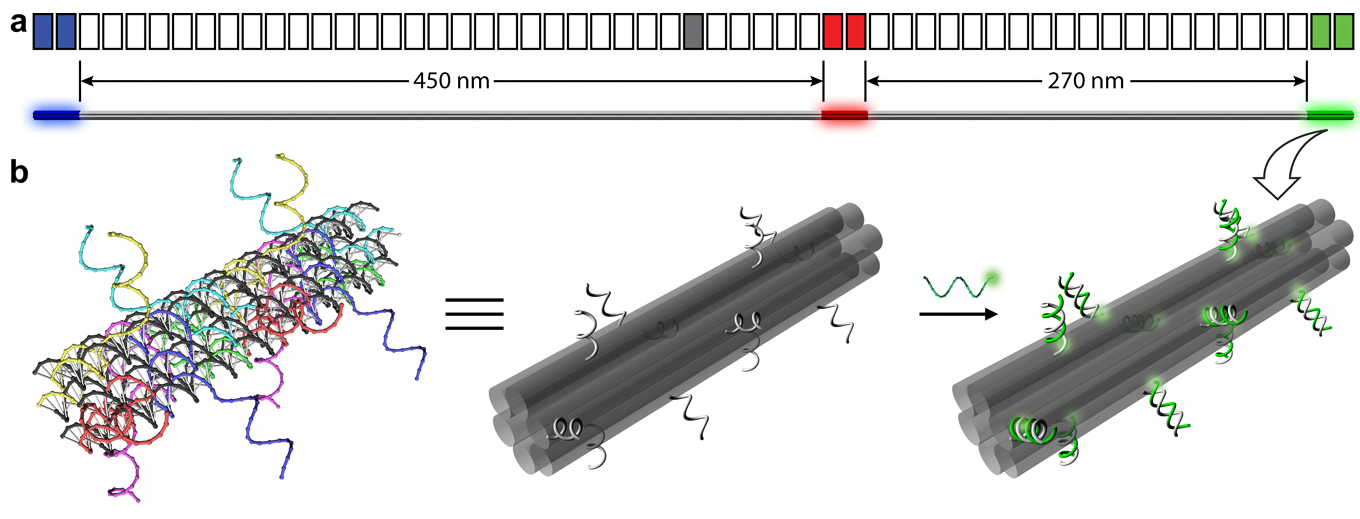
\includegraphics[width=\textwidth]{figures/dna1}
\caption[Design of the DNA-nanotube-based barcode.]{ Design of the DNA-nanotube-based barcode. (\textbf{a}) Two schematic drawings of 
the Blue--Red-Green (BRG, “--” and “-” denotes larger and smaller inter-zone distance in 
the barcode, respectively) barcode with a segment diagram on the top and a 3D view at 
the bottom. The main-body of the barcode is a DNA nanotube formed  by  
dimerizing two origami monomers, each consisting of 28 segments of length 42-bp (13.6 nm).
The grey segment in the middle represents the junction where the two monomers 
are joined together through cross-hybridization between their scaffolds and staples. Three 
84-bp zones of the nanotube are fluorescently labeled (shown as blue, red and green 
segments) to produce the BRG barcode with an inter-zone distance of 450 nm between 
the first two zones and 270 nm between the last two. Note that each zone is only labeled 
with one fluorophore species. The resulting barcodes are thus referred as single-labeled- 
zone barcodes. (\textbf{b}) 3D cartoons showing the details of one fluorescently labeled zone. 
Left: a scaffold-plus-staple model of such an 84-bp zone before labeling. Each of the 
twelve 63-base-long staples (shown in rainbow colors) contains two parts: the 42-base 
region at the 5'-end weaves through three double-helices to fold the scaffold (shown in 
black) into a six-helix bundle nanotube; and the 21-base extension at the 3'-end protrudes 
out for fluorescent labeling. Middle: an identical but simplified model to emphasize the 
six-helix bundle structure (each helix shown as a semi-transparent grey cylinder) and the 
positioning of the twelve 21-base staple extensions (each shown as a light-grey curl). 
Right: Cartoon representation of a “green” 84-bp zone. The labeling is achieved by 
hybridizing the Cy3 (shown the glowing green spheres at the 3'-ends) modified strands to 
the staple extensions.\label{fig:dna1}}
\end{figure}

\subsection{Construction of Simple Barcode}
We assembled the DNA-origami nanotubes following the protocol in \citep{douglas_dna-nanotube-induced_2007} with slight experimental modifications (See Materials and Methods in SI). 
Briefly, two structurally identical but chemically distinct nanotube monomers (\textasciitilde400 nm 
each) were assembled in two separate test tubes by slowly cooling a mixture of 7.3-kb 
scaffold strands and a set of \textasciitilde200 staple strands from 80 \textdegree C to 24 \textdegree C over 15 hours. After 
folding, excessive staple strands were removed from the folded nanotubes through 
polyethylene glycol fractionation. The nanotube monomers were then incubated with the 
desired fluorescently modified oligonucleotides and the labeled monomers were mixed at 
an equimolar ratio to form the final barcode structure. The barcodes were subsequently 
purified via agarose-gel electrophoresis and immobilized on streptavidin-coated 
coverslips before imaging with epi-fluorescence (Supplementary Figure S.1.2) or TIRF microscopy (Figure 
\ref{fig:dna2} and \ref{fig:dna3}) in the presence of oxygen scavenging reagents \citep{liedl_self-assembly_2010}. 

\begin{figure} %2`
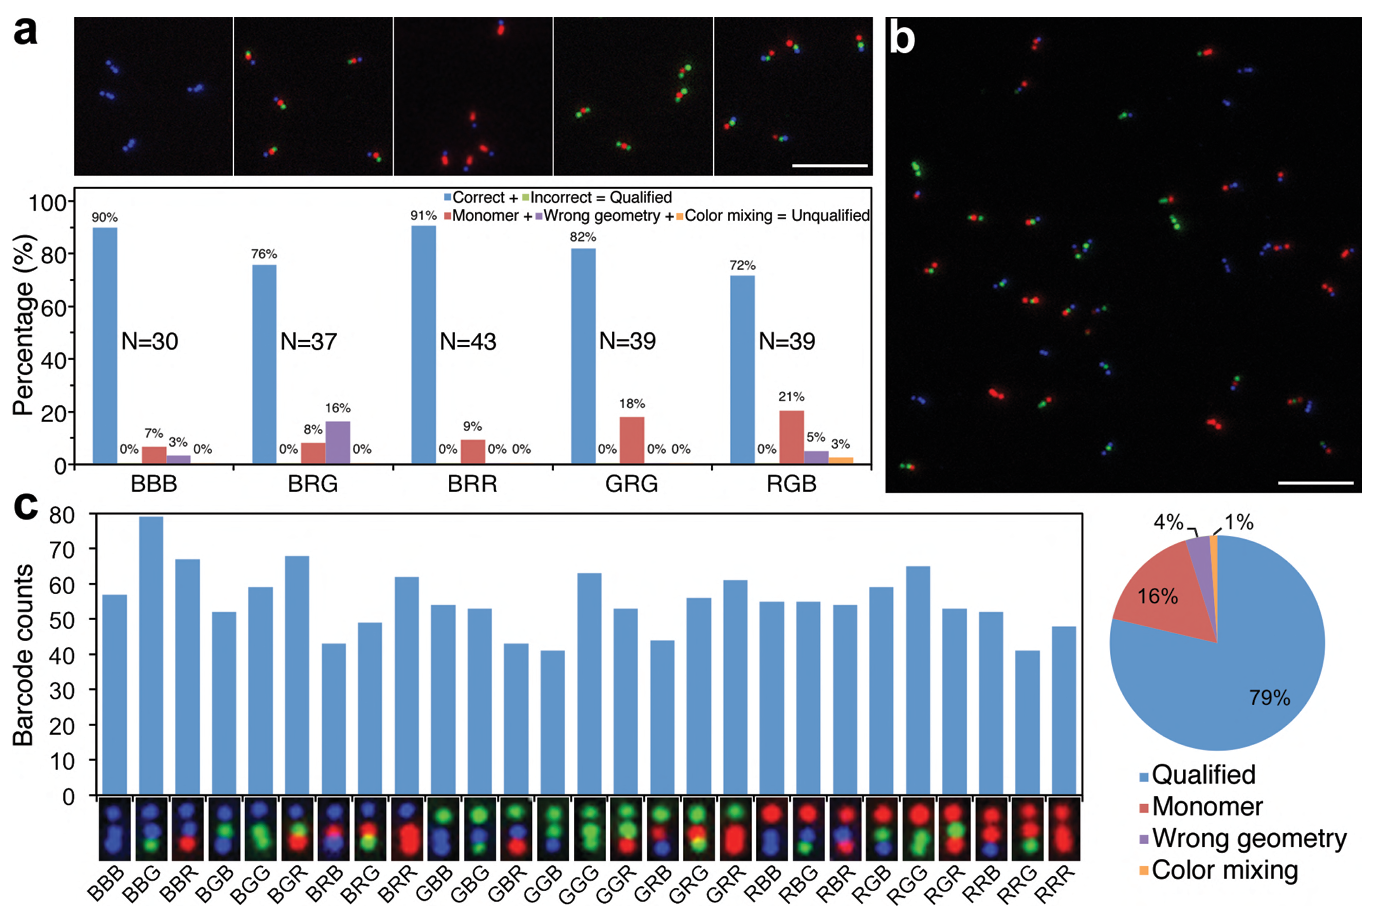
\includegraphics[width=\textwidth]{figures/dna2}
\caption[Single-labeled-zone fluorescent barcodes.]{Single-labeled-zone fluorescent barcodes. (\textbf{a}) Superimposed TIRF microscopy 
images of five barcode species (top) and the statistics from manual counting (bottom). 
From left to right are the BBB, BRG, BRR, GRG and RGB barcodes with a 
representative image on top of the corresponding bar-graph. Each bar-graph is generated 
based on the manual sorting and counting of the objects found in a 50×50 \textmu m$^2$ image 
(\textasciitilde40 barcodes, the exact sample size N is noted beside the corresponding bar-graph). (\textbf{b}) 
A representative image of the equimolar mixture of 27 barcode species. (\textbf{c}) Statistics 
obtained by analyzing twenty-seven 50×50 \textmu m$^2$ images of the 27 barcode mixture 
(\textasciitilde1,500 barcodes in total). Left: barcode counts of the 27 species (average count of 55 
with a standard deviation of 9). A representative TIRF image (1.4×0.7 \textmu m$^2$) of each 
barcode type is placed underneath the corresponding bar. Right: sorting result of the 
observed objects shown as a pie-chart. Color scheme used for the bar-graphs and the pie- 
chart (unrelated to the pseudo-colors of the fluorophores): blue, correct barcodes 
(qualified barcode with expected identity); green, incorrect barcodes (qualified barcode 
with unexpected identity); red, monomer nanotubes (one spot or two connecting spots); 
purple, barcodes with wrong geometry (i.e., bending angle <120\textdegree, see methods in SI); 
and orange, barcodes containing at least one spot with two colors. Note that in the 27- 
barcode pool, correct vs. incorrect barcodes were not distinguishable because all barcode 
types are expected. As a result the bars and pie representing the qualified barcodes in (\textbf{c}) 
are shown in blue. Scale bars: 5 \textmu m.\label{fig:dna2}}
\end{figure}
	

\subsection{Inspecting the simple barcodes}
In order to validate our system, we randomly chose five distinct barcodes from the
%Note to Chenxiang: What does it mean to "validate" the system? what specifically are you doing this section?
% Aren't you really just inspecting the barcodes and confrimng that they look as expected?
27 members in the barcode family for quality control experiments. The barcodes were 
assembled and purified separately and imaged under the same experimental conditions. 
Two distinct features of the barcode were clearly visible from the TIRF images (Figure 
\ref{fig:dna2}a, top panel and Supplementary Figure S.1.3): first, each fluorescently labeled zone on a barcode was 
resolved as a single-color spot and each complete barcode consisted of three of such 
spots; second, two of the neighboring spots were separated by a small gap while the other 
two neighbors sat closely together. Therefore one can visually recognize and decode 
those geometrically encoded barcodes based on the color identity of the spots and their 
relative spatial positions, even without the aid of any specialized decoding software. 
Using a custom-written software that localizes the center of each spot on the BRG 
barcodes (Supplementary Figure 
S.1.4), we measured the average center-to-center distance between the 
neighboring spots to be 433$\pm$53 nm (mean$\pm$s.d., N=70; larger distance) and 264$\pm$52 nm 
(mean $\pm$ s.d., N=70; smaller distance), confirming the correct formation of the barcodes. 
These experimentally measured distances were slightly smaller than the designed values 
(478 nm and 298 nm). We attribute this discrepancy to random thermal bending of the 
nanotubes (persistence length of \textasciitilde1–2 \textmu m), which has been observed previously by 
others \citep{rothemund_folding_2006, han_folding_2010} and confirmed by us (Supplementary Figure S.1.5) using transmission electron microscopy 
(TEM). It is important to note that unlike some other geometrically encoded barcoding 
systems (e.g., NanoString nCounter \citep{geiss_direct_2008}), there was no molecular combing step involved in
%Note to Chenxiang: is this the best place to put hthe nanostring comparison? It disrupts the rest of the already long paragraph.
the sample preparation. The separation between the fluorescent spots was exclusively 
created by the inherently rigid structure of the six-helix bundle nanotube. It is also 
notable that the spot intensities were not perfectly uniform across the whole image, which 
can be explained by factors such as the uneven illumination of the sample stage and 
differences in labeling efficiency. Nevertheless, the TIRF images proved that the 
barcodes were successfully assembled and can be resolved unambiguously.

\subsection{Quantification of the yield of the simple barcodes}
We then %I added a paragraph break here -AML
manually investigated TIRF images with an area of 50×50 \textmu m$^2$ for the five selected 
barcodes (Figure \ref{fig:dna2}a, bottom panel). The objects found within the images were first sorted 
into qualified (i.e., three single-color spots arranged in a nearly linear and asymmetric 
fashion as designed) and unqualified (i.e., all other objects) barcodes. The qualified 
barcodes were further categorized into correct and incorrect (false-positive) barcodes 
based on the fluorescent signatures of the composing spots to reflect whether the barcode 
was the expected type. The unqualified barcodes were further sorted into (1) monomer 
nanotubes (single spot or two “kissing” spots), (2) barcodes with “wrong” geometry (i.e., 
extreme bending), and (3) barcodes containing at least one spot with multiple colors. Our 
statistics revealed that more than 70\% of the visible objects were qualified barcodes, 
which we further determined to be exclusively the expected type (i.e., zero false-positive 
out of 188 qualified barcodes observed). The unqualified barcodes likely arose from 
folding defects, sample damage during handling and overlapping nanotubes on the 
surface, which can be largely reduced by optimizing the sample preparation and imaging 
protocol. 

%strike "real-life" added "useful" --AML
To be useful for multiplexed imaging system, a number of different barcode species must
coexist in one pool. Thus it is important to examine the robustness of our system by 
mixing different types of barcode together. In an initial test, we synthesized BRG and 
RGB barcodes separately, mixed them together at equal molar ratio and co-purified them 
via gel electrophoresis. The TIRF analysis of the purified mixture (Figure S.1.6) confirmed 
the 1:1 stoichiometry of the two barcodes and the overall assembly success rate (qualified 
barcode/all objects) of \textasciitilde80\%, suggesting that both barcodes maintained their integrity in 
the mixing and co-purification process. In addition, over 98\% of the qualified barcodes 
fell into one of the two expected types (BRG and RGB). The 2\% false-positive rate was 
due to an unexpected barcode, namely BGB (Figure Supplementary S.1.6), which could be attributed to a 
rare occasion in which the front monomer of the BRG barcode lay in proximity to the 
rear monomer of the RGB barcode. We believe this could be eliminated in the future if a 
more stringent purification condition is applied to minimize the amount of leftover 
monomers.  


%We should do a better job with organization here.. this is a very very long section, without much direction. Perhaps we could make clear the different instances with which we will inspect barcodes...
We next inspect barcodes when all 27 members of the barcode family were mixed at equimolar amount. The TIRF images 
(Figure \ref{fig:dna2}b and Figure S.1.7) showed that all types of barcodes were resolved. Statistical 
analyses of twenty-seven 50×50 \textmu m$^2$ images (\textasciitilde1,500 barcodes in total) revealed an 
average count of 55 per barcode type with a standard deviation of 9 (Figure \ref{fig:dna2}c), fitting 
well with the expected stoichiometry considering pipetting and sampling errors. The 
distribution of observed objects over the four categories (note that here correct vs. 
incorrect barcodes were not distinguishable as all 27 types were included) was consistent 
with the values measured from the single-type barcode samples. The above observations 
suggest that the sub-micrometer-long DNA nanotube represents a reliable platform to 
construct geometrically encoded barcodes with built-in structural rigidity. 


\section{Dual-labeled DNA origami Barcodes}

\begin{FPfigure} %3
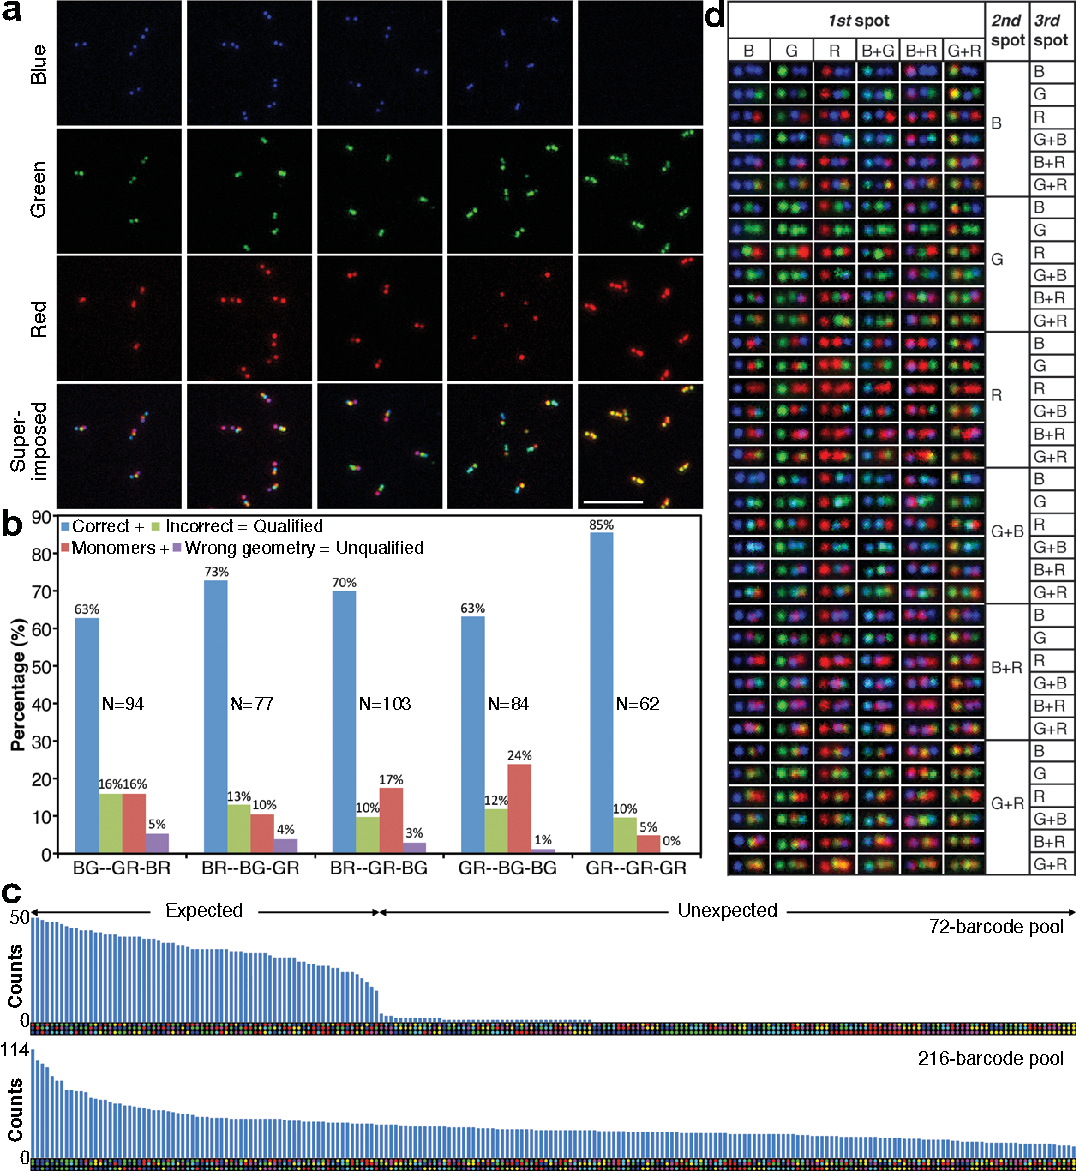
\includegraphics[width=\textwidth]{figures/dna3}
\caption[Dual-labeled-zone fluorescent barcodes.]{Dual-labeled-zone fluorescent barcodes. (\textbf{a}) Typical TIRF microscopy images 
of five selected barcode species, shown both in separate channels and after 
superimposing. Scale bar: 5 \textmu m. (\textbf{b}) Statistics obtained by analyzing two 50×50 \textmu m$^2$ 
images of each barcode species (\textasciitilde85 barcodes, the exact sample size N is noted beside 
the corresponding bar-graph). The barcode types are noted under the x-axis of the 
diagram. Color scheme (unrelated to the pseudo-colors of the fluorophores): blue, correct 
barcodes (correct geometry and color identity); green, incorrect barcodes (correct 
geometry but incorrect color identity); red, monomer nanotubes (one spot or two 
connecting spots); and purple, barcodes with wrong geometry (i.e., bending angle <120°, 
see methods in SI). (\textbf{c}) Computer-aided barcode counting results of the 72-barcode pool 
(N=2,617) and the 216-barcode pool (N=7,243) plotted as bar-graphs with descending 
barcode counts from left to right (see Supplementary Tables S.1.6 and S.1.7 for the numeric counting results). 
A computer-generated reference barcode image is placed underneath the corresponding 
bar. (\textbf{d}) A table containing one representative TIRF image (1.4×0.7 \textmu m$^2$) for each of the 
216 dual-labeled-zone barcode species. 
\label{fig:dna3}}
\end{FPfigure}


Our modular design enabled straightforward reengineering of the barcode to 
enhance its multiplexing capability through a variety of ways. For example, we changed 
the sequence of six staple extensions per zone so that instead of using twelve identical 
fluorescent oligonucleotides for labeling, we had the ability to use the combination of up 
to two fluorophores to create more unique fluorescence signatures (pseudo-colors) for 
%In the language of the introduction, this is an intensity strategy --AML
each zone. Six pseudo-colors (B, R, G, BG, BR, and GR) were generated by this “dual- 
labeling” strategy using three spectrally differentiable fluorophores. Consequently, the 
total number of distinct barcodes was raised from $3^3=27$ to $6^3=216$, which represented 
an order of magnitude increase in the multiplexing capability. 

\subsection{Inspecting the dual-labeled barcodes}
Similar to the single- 
labeled-zone barcode family, 5 members from the dual-labeled-zone barcode family were 
chosen for quality control purposes. The barcodes can be visually decoded either solely 
from the superimposed image or by examining all different channels simultaneously. For 
example, as shown in the first column of Figure \ref{fig:dna3}a, the barcode “BG--GR-BR” (“--” and 
“-” denotes larger and smaller inter-zone distance in the barcode, respectively) exhibits
two spots each in the blue, green and red channels but with descending gaps between 
them, matching its design. In the superimposed image, the barcodes are seen as Cyan-- 
Yellow-Pink, an expected consequence of color mixing caused by the dual-labeling 
strategy. In a similar fashion, we further verified the correct formation of the other four 
selected barcodes (Figure \ref{fig:dna3}a and Supplementary Figure S.1.8). Although the final pseudo-color from the dual- 
labeled zones was not always uniform (e.g., some yellow spots were green-tinted while 
the others were red-tinted) due to inconsistent labeling efficiency and minor sample 
displacement during imaging, the fluorescence signature of any given spot could be 
identified by checking the raw images acquired from the three imaging channels. We 
manually analyzed two 50×50 \textmu m$^2$ images of each dual-labeled-zone barcode and 
plotted the statistical data in Figure \ref{fig:dna3}b. Here, objects were sorted into qualified barcodes 
and unqualified barcodes based on their geometry and the qualified ones were further 
categorized as either correct or incorrect. We found that 75–95\% of the objects were 
qualified barcodes, among which 80–90\% were the correct type (percentage varies 
depending on the exact type of barcode). Compared to the single-labeled-zone barcode 
family, the percentage of qualified barcodes remained the same, while the false positive 
rate increased significantly from zero (Figure 1a) to 10–20.


%I am omitting a paragraph from the original text here --AML


We further tested the dual-labeled-zone barcoding system by imaging a mixture 
containing 72 barcode species that were individually assembled and co-purified (Supplementary Figure 
S.1.9). Custom MATLAB scripts were used to assist the decoding process (See Methods, Section \ref{sec:dna_Methods:Matlab}) in 
two steps. In step one, a three-channel (red, green, blue) TIRF image containing barcodes 
was pre-processed to remove background and thresholded so that only pixels containing 
qualified barcodes remained. The resulting three-channel binary image was merged to 
generate a single-channel binary image. Next, the software identified the location and 
orientation of geometrically legitimate barcodes based on their shape in the binary image. 
In step two, for each barcode located in step one, the corresponding region of the three- 
channel image was compared against a library of all possible reference barcodes. The 
observed barcode was assigned the identity of the reference barcode with the highest 
correlation. The fully automated decoding process (unsupervised mode) ended after the 
above two steps. In an optional supervised mode, the software presented the user with the 
observed barcode and its most likely identity for approval. Comparison between 
supervised and unsupervised decoding results confirmed >80\% agreement between the 
computer and the user (Supplementary Figure 
S.1.11). The computer-aided 
(supervised mode) analysis of thirty-six 64× 64 
 \textmu m$^2$ three-channel images registered 
\textasciitilde2,600 qualified barcodes that belonged to 116 different species (Table S.1.6 and Figure \ref{fig:dna3}c, 
top panel). The expected 72 species constituted \textasciitilde98\% of the total barcode population 
with an average barcode count of 36 per species and a standard deviation of 8. In 
contrast, the unexpected species averaged only \textasciitilde1.4 barcodes per species (maximum 4 
counts). Finally, we analyzed a mixture containing all the 216 members of the dual- 
labeled-zone barcode (Supplementary Figure S.1.12). Sixty 64× 
64 
 \textmu m$^2$
images of this mixture were 
processed by the decoding software in the unsupervised mode. The fully automated 
analysis registered a mean barcode count of \textasciitilde34 per species (\textasciitilde7,200 barcodes total) with 
a standard deviation of 17 (Table Supplementary Figure S.1.7 and Figure \ref{fig:dna3}c, bottom panel). Our study demonstrates that 216 
barcode species were successfully constructed and resolved (Figure \ref{fig:dna3}d). 


\section{DNA origami barcode system requiring super-resolution microscopy}
Increasing the number of spatially differentiable fluorescently labeled zones on 
the origami nanotube is another way to enhance the multiplexing capability of the 
barcoding system. A straightforward solution that keeps the inter-zone distances larger 
than the diffraction limit would require longer (e.g., a few micrometer long) nanotubes, 
which would likely result in lower assembly yield and decreased mechanical rigidity. 
Alternatively, one can add more fluorescently 
labeled zones on the ~800 nm tube and image the barcode using super-resolution 
fluorescence microscopy. As a feasibility demonstration of the latter approach, we 
applied DNA-PAINT \citep{jungmann_single-molecule_2010}, a recently developed super-resolution fluorescence technique, to 
image the barcodes. 

\subsection{Introduction to super-resolution microscopy techniques}
Over the last years, several techniques have been developed that 
allow imaging beyond the diffraction limit using far-field fluorescence microscopy \citep{hell_far-field_2007,hell_microscopy_2009,huang_breaking_2010,vogelsang_make_2010,walter_-it-yourself_2008}. 
In most super-resolution implementations, fluorophores are switched between 
fluorescence ON- and OFF-states, so that individual molecules can be localized 
consecutively. In methods relying on targeted readout schemes such as in Stimulated 
Emission Depletion Microscopy  (STED) \citep{hell_breaking_1994} or other Reversible Saturable Optical 
Fluorescence Transitions  (RESOLFT) techniques \citep{hell_far-field_2007}, fluorescence emission is actively 
confined to an area below the diffraction limit. The switching of fluorescent molecules 
can also be carried out stochastically such as in (direct) Stochastic Optical Reconstruction 
Microscopy \citep{heilemann_subdiffraction-resolution_2008,rust_sub-diffraction-limit_2006} (STORM, dSTORM), Photoactivated Localization Microscopy \citep{betzig_imaging_2006}
(PALM) and Blink Microscopy (BM) \citep{steinhauer_superresolution_2008}, where most fluorescent molecules are 
“prepared” in a dark state and only stochastically switched on to emit fluorescence. In 
Point Accumulation for Imaging in Nanoscale Topography (PAINT) \citep{sharonov_wide-field_2006}, fluorescence 
switching is obtained by targeting a surface with fluorescent molecules. In all stochastic 
approaches, fluorescence from single molecules is localized  in a diffraction-limited 
area to yield super-resolved images \citep{yildiz_myosin_2003,yildiz_kinesin_2004}.

DNA-PAINT uses transient binding of fluorescently labeled oligonucleotides 
(imager strands) to complementary “docking” strands on DNA nanostructures to obtain 
switching between a fluorescence ON- and OFF-state, which is necessary for 
localization-based super-resolution microscopy (See Figure \ref{fig:dna4}a). By adjusting the length of 
the imager/docking strand duplex and the concentration of imager strands in solution, 
fluorescence ON- and OFF-times can be tuned independently.

\subsection{DNA-PAINT-based DNA origami barcodes}
\begin{figure} %4
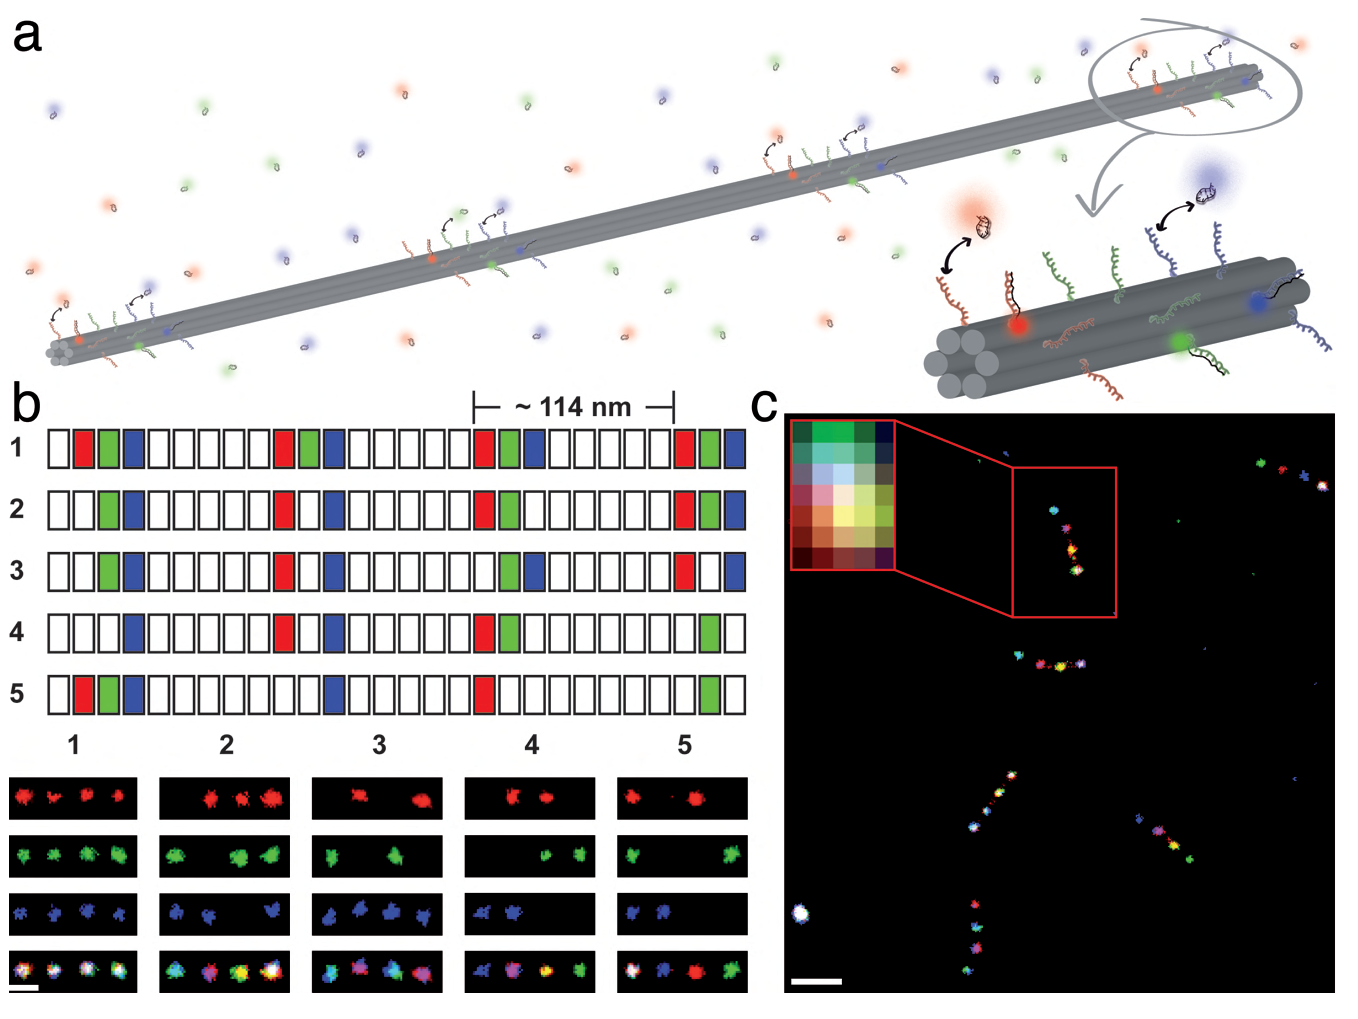
\includegraphics[width=\textwidth]{figures/dna4}
\caption[Super-resolution fluorescent barcodes.]{Super-resolution fluorescent barcodes.
 (\textbf{a}) Scheme of DNA-PAINT used for 
super-resolution barcode imaging. The 400 nm nanotube consists of 4 binding zones 
spaced by \textasciitilde114 nm. Each zone can be decorated with the desired combination of 
“docking” sequences for red, green or blue imager strands. The orthogonal imager strands 
bind transiently to their respective “docking” sites on the nanotube, creating the 
necessary “blinking” for super-resolution reconstruction (\textbf{b}) Top: segment diagram 
(similar to the one used in Figure \ref{fig:dna1}) of the DNA nanotube monomers used for creating 
five barcodes for super-resolution imaging. Bottom: super-resolution images of the five 
barcodes shown in each channel separately and as an overlay of all channels. Scale bar: 
100 nm. (\textbf{c}) Super-resolution image showing all five barcodes in one mixture. The inset 
shows the diffraction-limited image of one of the barcodes. Scale bar: 250 nm.
\label{fig:dna4}}
\end{figure}


For this study, we extended the DNA-PAINT technique to three-color imaging 
using orthogonal imager strand sequences coupled to three spectrally distinct dyes 
(Atto488 for blue, Cy3b for green and Atto655 for red excitation). To demonstrate the 
feasibility of the three-color super-resolution barcode system, we designed a DNA 
nanotube monomer with 4 binding zones in a symmetric arrangement. The neighboring 
zones were separated by \textasciitilde114 nm (i.e. well below the diffraction limit). Each binding 
zone consists of 18 staple strands, which can be extended to display three groups of 
orthogonal sequences (six per group) for the red, green or blue imager strands to bind. As 
a proof-of-principle experiment, we designed five different barcodes (Figure \ref{fig:dna4}a and top 
panel of b). The bottom panel of Figure \ref{fig:dna4}b shows the super-resolution reconstruction of 
the five barcodes for each channel separately as well as an overlay of all channels. Figure 
 \ref{fig:dna4}c shows a larger area containing all five barcodes. The unique pattern of the barcodes in 
all three channels can be resolved. Some of the barcodes can move during the sequential 
imaging (100 s acquisition time per channel) of all three color channels (see overview 
image in  Supplementary Figure 
S.1.14). Image conditions could still be improved by alternating excitation 
and faster image acquisition to prevent this effect. The transient, repetitive binding of 
imager strands to docking sequences on the nanotube not only creates the necessary 
"blinking" behavior for localization but also makes the imaging protocol more robust, as 
DNA-PAINT is not prone to photo-bleaching or incorrectly labeled strands (Supplementary Figure 
S.1.13). 
With the microscope setup we used, DNA-PAINT provides a resolution of \textasciitilde27 nm 
(FWHM of a Gaussian fit to the reconstructed PSF) in the red, \textasciitilde22 nm in the green and 
\textasciitilde23 nm in the blue channel. The obtainable resolution and imaging specificity suggests 
that 6 positions on one nanotube monomer could be robustly resolved while keeping the 
geometrical asymmetry of the barcode, which would lead to $7^6=117,649$ different 
possible barcodes. Furthermore the modularity of the nanotube design enables the 
customized reengineering of barcodes with inter-zone distances tailored to the resolving 
power of the used microscope, thus making it applicable for a wide range of microscope 
setups.

\section{More Complex Geometries}
DNA nanostructures with non-linear geometry could be assembled to generate 
more sophisticated barcodes. Figure 5 shows an example where three \textasciitilde400 nm DNA 
tubes were linked to the outer edge of a \textasciitilde60 nm DNA ring through hybridization between 
the staple extensions (Figure \ref{fig:dna5}a, inset). Fluorescently labeling the ring and the far end of 
the nanotubes generated a three-point-star-like structure clearly resolvable under 
fluorescence microscopy. TIRF microscopy and TEM studies (Figure \ref{fig:dna5}b, Supplementary Figures S.1.15 and S.1.16z) revealed that about 50\% of successfully folded barcodes featured three nanotubes 
surrounding the ring with a roughly 120\textdegree angle between each other as designed, while 
many other barcodes had significantly biased angles between neighboring nanotubes due 
to the semi-flexible double-stranded DNA linker between the ring and the nanotubes. It is 
conceivable that using similar design to connect three identical "satellite" linear barcodes 
to a central hub (here the three satellite barcodes may share the hub as a common 
fluorescently labeled zone), one can construct barcodes with triplicated encoding 
redundancy that feature outstanding reliability. In addition, more rigid linkers between 
the ring and the protrusions (e.g., multi-helix DNA with strand crossovers) could be 
employed to enforce better-defined barcode geometry. 


\begin{figure} %5
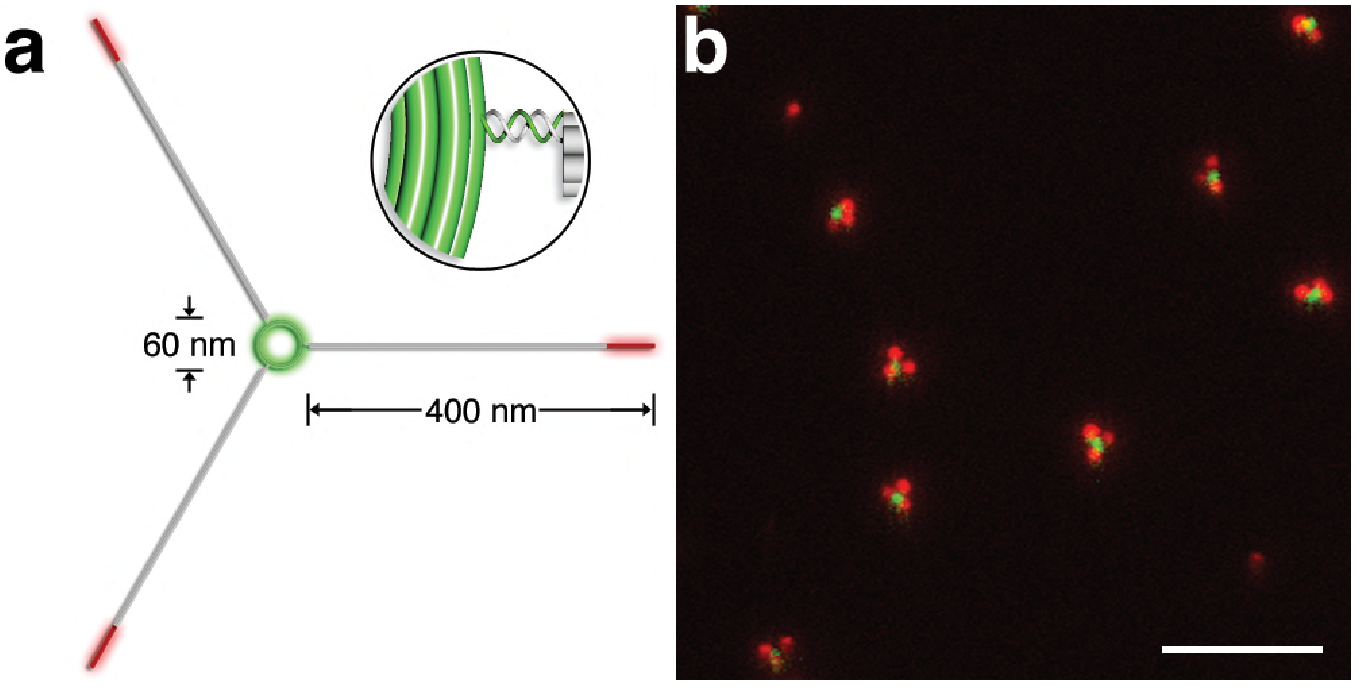
\includegraphics[width=\textwidth]{figures/dna5}
\caption[Fluorescent barcode with non-linear geometry.]{Fluorescent barcode with non-linear geometry. (\textbf{a}) Schematic. Three identical 
\textasciitilde400-nm long DNA nanotubes are linked to the outer edge of a DNA ring with diameter 
of \textasciitilde60 nm through the hybridization between staple extensions. The ring and the end of 
the tube are labeled by Cy3 (green) and Cy5 (red), respectively. (\textbf{b}) A representative 
TIRF microscope image of the barcode shown in (\textbf{a}). Scale bar: 5 \textmu m. 
\label{fig:dna5}}
\end{figure}



\subsection{DNA-PAINT-based DNA origami barcodes}

\section{DNA Barcodes attached to cells}
Modifying the barcodes with functional ligands such as antibodies and aptamers 
would allow the barcodes to tag specific biological samples and serve as multiplexed in 
situ imaging probes. In a proof-of-principle experiment, the GRG barcode was used to 
tag wild-type \textit{Candida albicans} yeast. The yeast cells were first mixed with a biotinylated 
polyclonal antibody specific to \textit{C. albicans}, then coated with a layer of streptavidin, and 
finally incubated with biotinylated GRG barcodes (Figure \ref{fig:dna6}a). TIRF microscopy revealed 
the barcodes attached to the bottom surface of the yeast cells (Figure  \ref{fig:dna6}b, top panel and 
Supplementary Figure S.1.17). While some of the nanotubes landed awkwardly on the uneven cell walls of 
the yeast cells, a number of GRG barcodes can be clearly visualized. In contrast, no 
barcode tagging was observed when non-biotinylated antibodies or barcodes were used to 
treat the yeasts (Figure  \ref{fig:dna6}b, bottom panel and Supplementary Figure 
S.1.17), suggesting that little to no non- 
specific interaction existed between the barcode and the cell surface. 

\begin{figure} %6
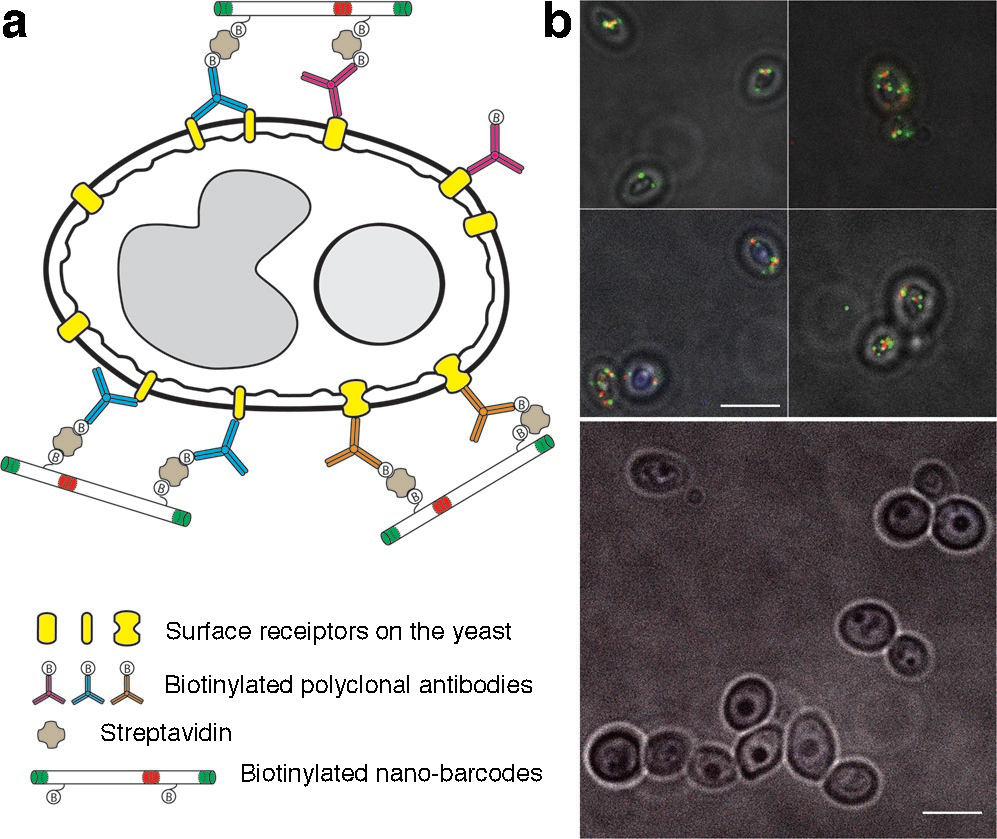
\includegraphics[width=\textwidth]{figures/dna6}
\caption[Tagging yeast cells with the GRG barcodes as \textit{in situ} imaging probes.]{Tagging yeast cells with the GRG barcodes as \textit{in situ} imaging probes. (\textbf{a}) 
Cartoon illustrating the tagging mechanism. The biotinylated barcodes are anchored on 
the yeast cell through streptavidin molecules bound to biotinylated polyclonal antibodies 
coated on the yeast surface. Only two of the ten biotinylated staples on the barcode are 
shown here for clarity. (\textbf{b}) Overlaid microscope images (acquired in bright field and 
TIRF) of the yeast cells treated with the barcodes. Top: yeast cells treated as illustrated in 
(\textbf{a}). Bottom: negative control: yeast cells treated with non-biotinylated barcodes. Scale 
bars: 5 \textmu m.
\label{fig:dna6}}
\end{figure}



\section{Discussion}
In summary, we have constructed a new kind of geometrically encoded 
fluorescent barcode using DNA-origami-based self-assembly. We took advantage of the 
mechanical rigidity of the multi-helix-bundle architecture, the addressable surface and 
spatial organizing power of the DNA-origami nanotube as well as the programmable 
linkage between multiple DNA nanostructures to build a modular, robust yet easy-to-
handle barcoding system. It differs from previously reported optically decodable 
barcoding systems in the following three aspects: First, and most notably, the DNA- 
origami-based barcodes are 400−800 nm in length, making them potentially useful to 
serve as \textit{in situ} single molecule imaging probes to tag sub-cellular entities such as surface 
protein markers (as demonstrated in the yeast tagging experiment), chromosomes, 
mitochondria and microtubules, which generally range from 500 nm to 20 \textmu m in size. 
Making use of the super-resolution barcode system, one could envision \textit{ex} and \textit{in situ} 
imaging of a wide variety of biomolecules such as mRNA or proteins simultaneously by 
using tagging techniques based on hybridization or SNAP tags \citep{gautier_engineered_2008,jones_fast_2011,keppler_general_2003,klein_live-cell_2011}. The system also 
fulfills a technological challenge to build robust finite-size optical barcodes with its 
smallest feature approaching or even smaller than the diffraction limit of visible light. 
Second, the barcodes presented here are massively self-assembled in parallel (typically 
1011 molecules per barcode species in one 50 \textmu L folding reaction) exclusively through 
DNA hybridization. Unlike previous constructions, the synthesizing and purification 
process requires no enzymatic reaction \citep{geiss_direct_2008}, genomic engineering \citep{livet_transgenic_2007}, photolithography \citep{pregibon_multifunctional_2007}, 
electrochemical etching \citep{cunin_biomolecular_2002} or microfluidic devices \citep{fournier-bidoz_facile_2008, pregibon_multifunctional_2007}, which makes the barcodes easy to 
reproduce in a typical biochemistry lab. The barcodes could be functionalized to display 
sequence-specific probes simply through DNA-origami staple extensions. Third, the 
robustness and programmability of the DNA-origami-based platform allows us to achieve 
high multiplexing capability. 

Here we successfully constructed 216 barcode species that 
were decoded in one pool, while the previously reported sub-micrometer-sized 
fluorescent barcodes contained no more than 11 distinct barcodes \citep{li_multiplexed_2005, fournier-bidoz_facile_2008, li_controlled_2010, levsky_single-cell_2002}. Even compared 
to the prior art of producing multi-color fluorescent barcodes that are less than 10 \textmu m in 
size, our system is among the few examples \citep{fournier-bidoz_facile_2008, geiss_direct_2008} that demonstrated more than 100 codes in 
practice. To the best of our knowledge, the only system that demonstrated larger numbers 
of barcodes coexisting in a homogenous solution is the NanoString nCounter \citep{ geiss_direct_2008}. However 
the reporter probes of the NanoString (\textasciitilde7-kb double-stranded RNA-DNA-hybrid 
molecules) require combing to make the codes resolvable, making them fundamentally 
unsuitable as \textit{in situ} imaging probes. In contrast, the DNA-origami-based barcodes 
maintain their structural integrity when applied to cell surfaces, suggesting their 
promising application as \textit{in situ} imaging makers. Furthermore, the combination of the 
DNA-PAINT imaging technique and the DNA-origami-based nanotubes allowed us to 
create the first nanoscopic "super-resolution" barcodes while maintaining the 
multiplexing power. To give an idea of the number of achievable different codes  
consider the incorporation of 12 fluorescently labeled zones into the 800-nm long dimer 
nanotube and using all possible equimolar combinations of the RGB fluorophores - an 
enormous number ($7^{12}\approx 1.4  \times 10^17$ of barcode
species can be generated. Using DNA- 
PAINT as a readout technique also makes the system less prone to fluorescent labeling 
errors, as the "imager strands" are replenished from solution during the acquisition 
process. Finally, the fact that the barcodes can be resolved using epi-fluorescence 
microscopy makes them more adaptive and implies their possible application in deep 
tissue labeling in the future. 

\section{Future Directions}
We note that the barcode design and experimental procedures can be refined to 
further minimize the false-positive rate of the dual-labeled-zone barcodes. For example, 
fluorophores with higher quantum efficiency and less susceptibility to photobleaching 
(e.g. Atto dyes or quantum dots) could be used to improve imaging quality. Higher 
quality staples (e.g., enzymatically produced and HPLC purified) could be used to fold 
the barcode to enhance fluorescent labeling efficiency by minimizing the number of 
missing or truncated staple extensions in the binding zones. Barcodes could be purified 
under more gentle conditions (e.g., recover DNA from agarose gel through electro- 
elution \citep{bellot_recovery_2011} instead of crush-and-soak) to reduce the possibility of breaking a dimer 
nanotube into two monomers. The purified barcodes could be chemically cross-linked \citep{rajendran_photo-cross-linking-assisted_2011}
to improve their thermal and mechanical stability. Redundant coding could be built into 
the barcode to generate more reliable readouts. In practice, it is likely that a small number 
of distinct codes could be sufficient to label the targets of interests. For those 
applications, one could selectively use the most robust subset of the barcode library. A 
larger library of barcodes may be achieved through more sophisticated geometrical and 
intensity encoding, which is made possible by our growing ability to build more 
complicated DNA nanostructures and to optically resolve features below the diffraction 
limit. At the same time, as computational power and image-processing technology 
advance, future barcode analysis systems should run more accurately. In the future, we 
expect our barcode technology to interface with the rapidly growing protein/antibody 
library technology to yield a powerful imaging toolbox for single-molecule studies of 
biological events and biomedical diagnostics. 


\section{Materials and Methods}
\subsection{Materials}
Non-modified DNA Oligonucleotides were purchased from Bioneer Inc. (Alameda, CA). Fluorescently modified DNA oligonucleotides were purchased from Integrated DNA Technology (Coralville, IA) and Biosynthesis (Lewisville, TX). Polyclonal antibodies to C. albicans were purchased from Thermo Scientific (Rockford, IL). Streptavidin was purchased from Invitrogen (Carlsbad, CA). Glass slides and coverslips were purchased from VWR (Radnor, PA). All other reagents were purchased from Sigma-Aldrich (St. Louis, MO). M13mp18 scaffold strand for the DNA origami drift markers was obtained from New England Biolabs (Ipswich, MA).
Design of the nano-barcodes
The main-body of the linear nano-barcode is a DNA six-helix-bundle (6hb) nanotube dimer designed using the caDNAno software (\url{http://cadnano.org}). The structure of the barcode is illustrated as a strand diagram in Figure S.1.1. Staples in the fluorescent labeling zones were extended at the 3'-end with 21-base long single-stranded overhangs (handles) for fluorescent labeling (see table S.1.1 for staple extension sequences). In addition, ten staples (five per monomer, shown as magenta strands in the diagram) were extended at the 5'-end with biotin. The three-point-star like barcode is self-assembled from three identical DNA 6hb nanotube monomers and a DNA 6hb ring. Here, 12 handles protrude out from a helix on the outer edge of the ring. Three of them serve as sticky-ends to link with the 6hb nanotubes while the other nine are used for fluorescent labeling. The 6hb nanotube carries a handle at the front end to serve as the complementary sticky-end and 24 handles at the rear end for fluorescent labeling. The design is illustrated as a strand diagram in Figure S.1.1 and the staple extension sequences used in this design are listed in table S.1.2.

\subsection{Self-assembly of the nano-barcodes}
To fold the \textasciitilde800 nm DNA-nanotube based barcode, the monomer nanotubes were each assembled and fluorescently labeled in a separate test tube and then mixed together to form the dimer. The assembly of the monomer was accomplished in one-pot reaction by mixing 100 nM scaffold strands (7,308-base long, termed p7308, see table S.1.4 for sequence) derived from M13 bacteriophage with a pool of oligonucleotide staple strands (600 nM of each; reverse-phase cartridge purified.) in folding buffer containing 5 mM Tris, 1 mM EDTA, 20 mM MgCl$_2$, 50 mM NaCl (pH 8) and subjecting the mixture to a thermal-annealing ramp that cooled from 80 \textdegree C to 60 \textdegree C over the course of 80 minutes and then cooled from 60 \textdegree C to 24 \textdegree C over 15 hours. Excessive staples were removed from the folded nanotubes by polyethylene glycol fractionation \citep{lis_size_1975}.

 To fluorescently label the nanotubes, desired DNA oligonucleotides with complementary sequence to the handles (termed anti-handles, see table S.1.3 for sequences) were added to the monomers (1.2:1 molar ratio between anti-handles and handles) and the hybridization was carried out at 37 \textdegree C for 2 hours. For dimerization, stoichiometric amount of the two fluorescently labeled monomers were mixed and incubated at 16 \textdegree C overnight. The final product was loaded on a non-denaturing, 1.5\% agarose gel and electrophoresed at 3V/cm in ice-cold 0.5× TBE buffer containing 10 mM MgCl$_2$ for 3.5 hours. It is important not to expose the fluorescently labeled nanotube dimers to elevated temperature (>25\textdegree C) to avoid the cross-contamination because some handles in different fluorescent labeling zones share the same oligonucleotide sequence (Table S.1.1). The desired band was excised and the nanotube dimers were recovered from the agarose gel using a pellet-pestle method \citep{kurien_extraction_2002}. To prepare an equimolar mixture of 2, 27, 72 or 216 barcodes, all the barcode species involved are folded, labeled and dimerized separately and then mixed at equal molar ratio for agarose gel electrophoresis purification. To produce the three-point-star like barcode, the DNA nanotube was folded and labeled as described above and the DNA ring was prepared under similar conditions, with the p3024 scaffold (3,024-base long circular ssDNA derived from pBluescript vector, see table S.1.4 for sequence), staple and MgCl$_2$ concentration changed to 25 nM, 125 nM (each) and 10 mM, respectively. The labeled ring and the nanotube were then purified separately through agarose gel electrophoresis, mixed together at 1:3 molar ratio and incubated at 37 \textdegree C overnight. The final product was purified via gel electrophoresis as described above.

\subsection{Tagging yeast cells with nano-barcodes}
Approximately  C. albicans yeast cells were suspended in 150 \textmu L of PBS buffer ( cells per microliter). 1 \textmu L of 4 mg/mL polyclonal antibody (with or without biotin label) was added to this suspension and allowed to bind to the cell surface for 15 minutes. The yeasts were then spun in a desktop centrifuge at 4000 rcf for 15 minutes to form a pellet and washed with 150 \textmu L of PBS buffer twice. The antibody-coated cells was then resuspended in 150 \textmu L of PBS buffer and mixed with 2 \textmu L of 10 mg/mL streptavidin. After incubating for 10 minutes, the cells were again spun and washed as described above. The cell pellet was then resuspended in 150 \textmu L of PBS buffer containing 10 mM MgCl$_2$ and 0.05\% Tween-20 (termed PBS+ buffer here) and treated with 2 \textmu L of 2 nM biotinylated or non-biotinylated GRG nano-barcode. After 30 minutes incubation on a desktop shaker, the yeast cells were pelleted and washed three times with 150 \textmu L of PBS+ buffer.

\subsection{Sample preparation for fluorescence imaging}
A piece of coverslip (No. 1.5, 18  18 mm$^2$, \textasciitilde0.17 mm thick) and a glass slide (3  1 inch$^2$, 1 mm thick) were sandwiched together by two strips of double-side tapes to form a flow chamber with inner volume of \textasciitilde15 \textmu L. First, 20 \textmu L of biotin labeled bovine albumin (1 mg/mL, dissolved in Buffer A (10 mM Tris-HCl, 100 mM NaCl, 0.05\% Tween-20, pH 7.5)) was flown into the chamber and incubated for 2 minutes. The chamber was then washed using 20 \textmu L of Buffer A twice. 20 \textmu L of streptavidin (0.5 mg/mL, dissolved in Buffer A) was then flown through the chamber and allowed to bind for 2 minutes. After washing twice with 20 \textmu L of Buffer B (5 mM Tris-HCl, 10 mM MgCl$_2$, 1 mM EDTA, 0.05\% Tween-20 pH 8, supplemented with 2.5 mM protocatechuic acid, 10 nM protocatechuate-3,4-dioxygenase and 1 mM Trolox), 20 \textmu L of biotin labeled nano-barcodes (10 pM in Buffer B) were finally flown into the chamber and incubated for 2 minutes. The chamber was washed using 20 \textmu L of buffer B for three times, sealed with nail polish and mounted on the sample stage of a microscope with the coverslip facing towards the objective. For DNA-PAINT imaging, samples were prepared as described above. The final imaging buffer solution contained 20 nM ATTO488, Cy3b and ATTO655 labeled imager strands in Buffer B respectively. For the three-point-star shape barcode and the yeast cells, 5 \textmu L of specimen was directly deposited on the glass slide, covered immediately with a piece of coverslip, sealed with nail polish and incubated for 5 min before mounting onto the sample stage. 

\subsection{Diffraction-limited fluorescence imaging}
Fluorescence imaging was carried out on an inverted Leica DM1600B microscope (Buffalo Grove, IL) applying an objective-type TIRF configuration using a Leica TIRF illuminator with an oil-immersion objective (HCX PL APO 100/1.47 oil CORR TIRF). Additional lenses were used to achieve a final imaging magnification of \textasciitilde112 fold, corresponding to a pixel size of \textasciitilde71 nm. A 488 nm solid state laser (JDS Uniphase, FCD 488-10), a 561 nm solid state laser (LASOS YLK6110) and a 635 nm diode laser (BSR, ChromaLase 635) were used for TIRF excitation. Laser beams were filtered with clean up filters (zet488x, zet561x, 635x) and coupled into the microscope objective using a multi-band beamsplitter (zt488, zt561, zt635). Fluorescence light was spectrally filtered with emission filters (ET525/36, ET600/32, ET705/72) and imaged on an EMCCD camera (Hamamatsu C9100-02, Hamamatsu, Japan). Exposure times were 1 second for 488 nm excitation and 700 ms for 561 and 635 nm excitations. Two consecutive images were taken for the same area of sample and then averaged to yield the final image. The laser beam alignment and imaging process were automatically controlled by the Leica LAS software. The TIRF images were processed using ImageJ and a custom written software for decoding (see the decoding software section).

For epi-fluorescence imaging, the full-spectrum light generated from a mercury lamp was filtered through desired filters (470/40, 560/40 and 645/30 for blue, green and red channel, respectively) to serve as excitation source. The same beam splitter and emission filters were used as in the TIRF mode. The exposure time for all channels was 2 seconds. For the barcode treated yeast sample, an additional bright field image was taken to show the profile of the cells. 

\subsection{DNA-PAINT Imaging}
Super-resolution fluorescence imaging using DNA-PAINT was carried out on two different microscope systems. Figure 4 and Figure S.1.14 were acquired on an inverted Zeiss LSM 710 ELYRA PS.1 microscope (Carl Zeiss, Germany) applying an objective-type total internal reflection fluorescence (TIRF) configuration using an oil immersion objective (100x alpha Plan Apo, NA 1.46, Oil, Zeiss). An additional 1.6 magnification was used to obtain a final imaging magnification of \textasciitilde160 fold, corresponding to a pixel size of 100 nm. Samples were imaged using custom made microscopic chambers. Three lasers ($\lambda$=488 nm, 100 mW, $\lambda$=561 nm, 100 mW and $\lambda$=642 nm, 100 mW) were used for TIRF excitation. The laser beam was coupled into the microscope objective using a multi-band beamsplitter. Fluorescence light was spectrally filtered with an emission filter (BP 495-575/LP 750 for ATTO488 imaging, BP 570-65-/LP 750 for Cy3b imaging and LP 655 for ATTO655 imaging) and imaged on an EMCCD camera (Andor iXon 3, Andor Technologies, North Ireland). 5000 frames were recorded at a frame rate of 50 Hz for each color channel sequentially.

Figure S.1.13 was acquired on an inverted Nikon Ti-E microscope (Nikon Instruments, Melville, NY) with the Perfect Focus System, applying an objective-type TIRF configuration using a Nikon TIRF illuminator with an oil-immersion objective (100 Plan Apo, NA 1.49, Oil, Nikon). An additional 1.5 magnification was used to obtain a final imaging magnification of \textasciitilde150 fold, corresponding to a pixel size of 107 nm. Three lasers ($\lambda$=491 nm, 100 mW, $\lambda$=561 nm, 75 mW and $\lambda$=640 nm, 30 mW, BSR) were used for TIRF excitation. The laser beam was filtered with a clean up filter (488/20 for ATTO488 imaging, 561/20 for Cy3b imaging and 642/20 for ATTO655 imaging, all Chroma Technologies) and coupled into the microscope objective using a multi-band beamsplitter (zt405/488-491/561/638rpc, Chroma Technologies). Fluorescence light was spectrally filtered with an emission filter (525/50 for ATTO488 imaging, 600/50 for Cy3b imaging and 700/75 for ATTO655 imaging, all Chroma Technologies) and imaged on an EMCCD camera (Hamamatsu ImagEM C-9100-13, Hamamatsu, Japan). 5000 frames were recorded at a frame rate of 10 Hz for each color channel sequentially. 

Super-resolution images were reconstructed using spot-finding and 2-dimensional Gaussian fitting algorithms programmed in LabVIEW \citep{steinhauer_superresolution_2008}. A simplified version of this software is available for download at \url{www.e14.ph.tum.de}. Images were drift corrected and the different channels aligned using DNA origami drift markers with binding sites for all three imager strands (see Figure S.1.1d). The origami structure is based on Rothemund’s rectangular shaped origami	\citep{rothemund_folding_2006}. The black staple strands in the strand diagram were randomly extended with 2 out of three docking/handle strands for DNA-PAINT imaging. The resulting structure displays \textasciitilde80 binding sites on average for the red, green and blue imager strands respectively. This high density of binding sites yields to a constantly “occupied” i.e. bound state of one or more imager strands at every given moment in time. This makes the structures ideal for systematic drift correction in each channel and because the structures are imaged in each channel at the same positions, they can be used to correct for offsets and align the red, green and blue channel accordingly. 

\subsection{Automated characterization of the geometry of BRG and GRG barcodes}
For the purpose of assessing the barcode geometry, we chose BRG and GRG barcodes as examples. The software first determined the centroids of all visible spots in the diffraction limited TIRF images based on their fluorescence intensities. The centroid of a spot was defined as the brightest central pixel in a 3-pixel by 3-pixel region. The software processed blue, green and red fluorescence channels independently to identify all the centroids in each channel (Figure S.1.4). It then superimposed the three channels and found the correct barcodes based on the design blueprint. The distances between the neighboring fluorescently labeled zones were calculated as the distances between the centroids of the adjacent spots on a barcode. The barcode bending angle (a) was calculated using the cosine formula as shown below, where a and b are the distances between neighboring centroids and c is the distance between the farthest two centroids within a barcode. The measured parameters are listed in Table S.1.5.



\subsection{Decoding software for diffraction-limited TIRF images}\label{sec:dna_Methods:Matlab}
Custom MATLAB scripts were used to decode barcodes from diffraction-limited TIRF images. The software can run in either a supervised or an unsupervised mode. In the supervised mode, each decoded barcode is presented to the user to accept or reject. In unsupervised mode, the software decodes all barcodes without any user input.

The software operates in two steps: In the first step the software identifies the location and position of barcodes. In the second step the software actually decodes the barcode (See Figure \ref{fig:dna_MatlabBlockDiagram}). For step one, the software preprocesses the three-channel TIRF image containing the barcodes (one channel each for fluorescence in the red, green and blue). The image is spatially high-pass filtered to remove slowly spatially varying illumination background. Each color channel is then thresholded independently so that only pixels corresponding to putative barcodes remain. The three-channel thresholded image is then merged to generate a single channel binary image. The software identifies shapes from the binary image that match the length and width criteria of a barcode. The position and orientation of these shapes are recorded. In step two, the software reads each barcode identified in step one. For each barcode, the software extracts the corresponding region of the original three-channel image. This constitutes the observed barcode. The software then performs a matched filter to compare the observed barcode against a library of all possible reference barcodes. For each reference, three simultaneous correlations are performed, one in each color channel, while keeping all channels aligned. To reduce computations, these correlations are actually performed on one-dimensional projections of the 2D image of the observed barcode in each channel, so that each fluorescent spot appears as a peak in a 1D trace. The observed barcode is assigned the identity of the reference barcode with the highest combined correlation across all three color channels. 

\begin{figure}
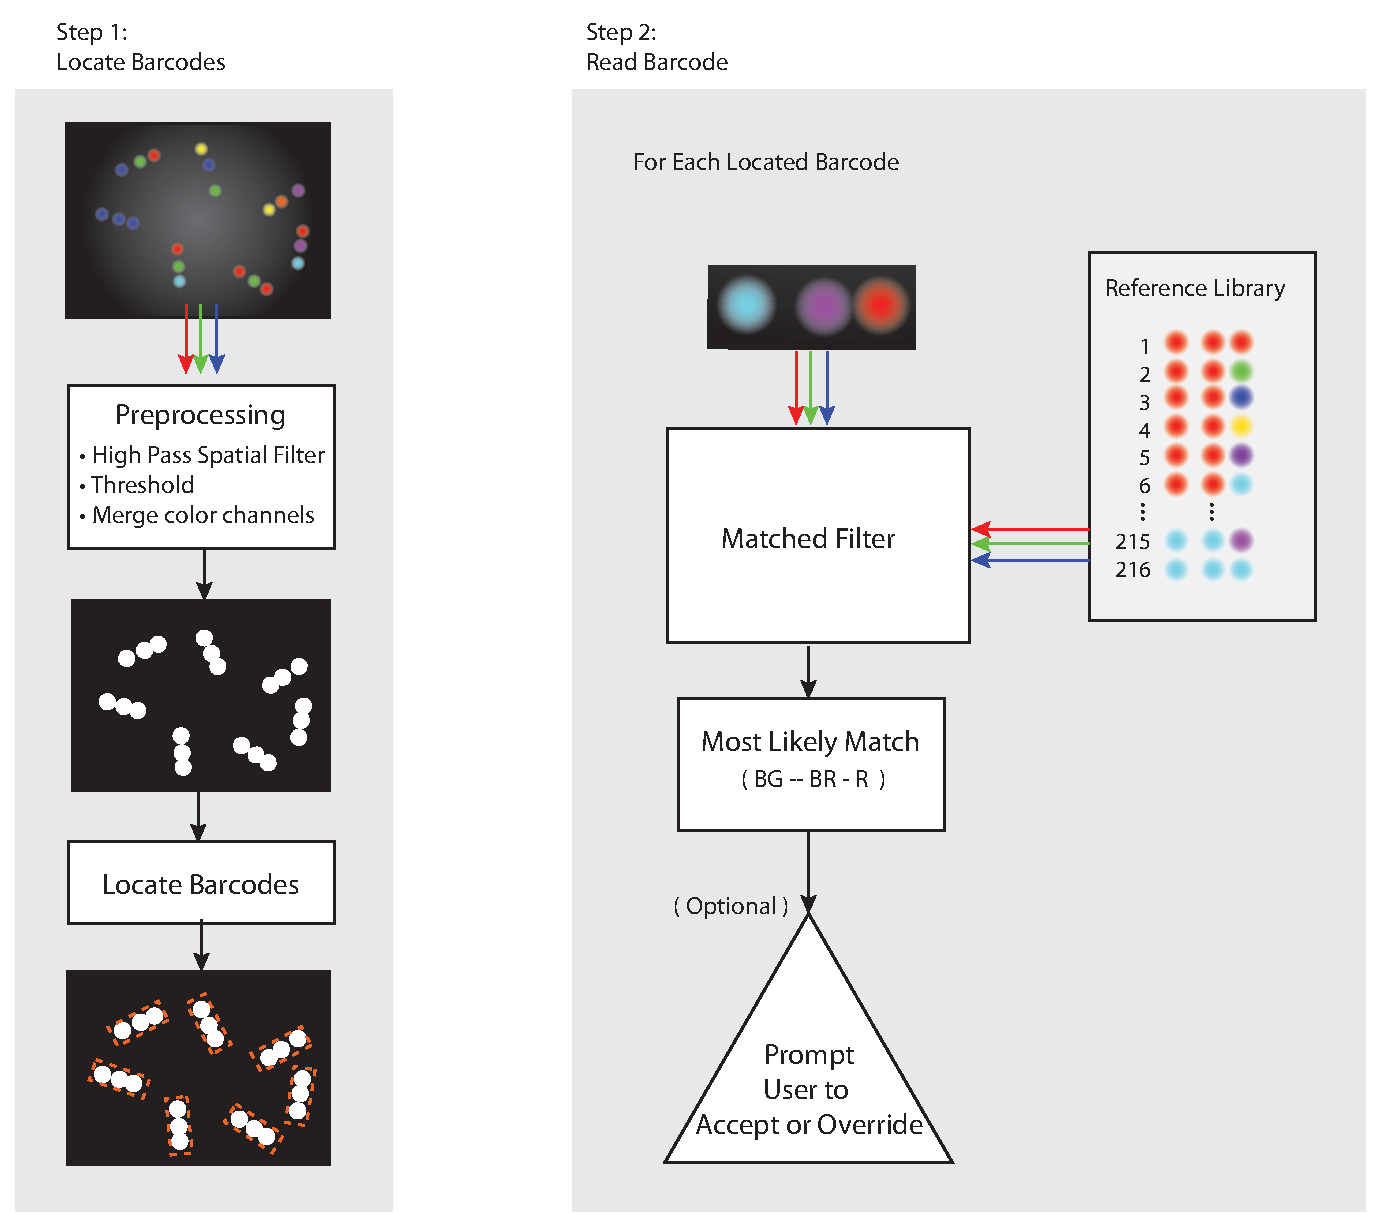
\includegraphics[width=\textwidth]{figures/dna_MatlabBlockDiagram}
\caption[Barcode anlaysis software]{
 Barcode analysis software box diagram. The MATLAB software operates in two steps: In the first step the software identifes the
location and position of barcodes. In the second step the software decodes the barcode  using a matched filter. 
\label{fig:dna_MatlabBlockDiagram}}
\end{figure}


When run in supervised mode, the computer will present the user with the image of the barcode and its most likely identity. The user can either accept the computers proposal or manually enter the correct identity of the barcode. In cases where the software erroneously decodes misshapen or malformed barcodes, the user can reject the barcode entirely. The software finally outputs the counts of all barcode species as well as the coordinates and identity of each individual barcode. When run in supervised mode, it also registers the number of occasions when the user approves the computer’s proposal. For the 72-barcode pool, this agreement rate is approximately 80\%.

\section{Acknowledgements}
We thank Dr. Christian Steinhauer and Sebastian Piet Laurien for help with super- 
resolution software development. We thank Dr. Bernhard Goetze and the Harvard Center 
for Biological Imaging as well as the Nikon Imaging Center at Harvard Medical School 
for the use of their microscopes. We thank Dr. Shawn M. Douglas for providing TEM 
images used in Supplementary Figure S.1.5. This work was supported by grants from an NIH Director’s New 
Innovator Award and a Wyss Institute for Biologically Inspired Engineering Faculty 
Award to W.M.S. and an NIH Director’s New Innovator Award, an NSF Faculty Early 
Development Award, an ONR Young Investigator Program Award, and Wyss Institute 
for Biologically Engineering Faculty Startup Fund to P.Y. R.J. acknowledges support 
from the Alexander von Humboldt-Foundation through a Feodor Lynen fellowship.


%Andy, don't forget to go back and add references to Supplementary Information and Supplementary Figures



\section{Manuscript Information}
\subsection{Submitted for Publication As}
A version of this chapter has been submitted for publication to the journal \textit{Nature Nanotechnologies}  as \citep{lin_sub-micrometer_2011},

\bibentry{lin_sub-micrometer_2011}.

\subsection{Author Contributions}
Andrew M.~Leifer designed and wrote the software to analyze TIRF images and identify and decode the barcodes. He wrote portions of the manuscript and generated Figure \ref{fig:dna_MatlabBlockDiagram}. This work lays the foundation for the more detailed analysis performed in Chapter \ref{chapter:DNAtheory}.

C. Lin conceived the project, designed and conducted the majority of the experiments, 
analyzed the data, and prepared the majority of the draft. R.J. conceived the super 
resolution barcode study, designed and conducted experiments for this study, analyzed 
the data, and prepared the draft. C. Li wrote the C script for the barcode 
geometry characterization. D.L. (with C. Lin) performed the yeast tagging experiment. 
W.M.S. conceived the project, discussed the results, and prepared the draft. P.Y. 
conceived, designed, and supervised the study, interpreted the data, and prepared the 
draft. All authors reviewed and approved the draft. 


\section{Supplementary Material}
 All Supplementary Tables and Figures are located in \texttt{Chapter5Supplementary.pdf} on the accompanying CD-ROM. 